In this section we illustrate comparative properties of group lasso, GrOWL-I and GrOWL-II by applying these to the analysis of synthetic data generated from a simple neural network motivated by the triangle model of word-reading (Figure \ref{fig.network} top left). This feed-forward network takes a model analog of word spelling as input (orthographic layer) and is trained to generate distributed representations of its meaning (semantic layer) and pronunciation (phonological layer). The network is deep in that mappings from orthography to phonology, from orthography to semantics, and from semantics to phonology, are all mediated by one or more hidden layers of units. The model's ability to generate phonological output is mediated by two separate pathways: a {\em direct} route mediated by a single hidden layer, and an "indrect" route composed of three hidden layers, which must first compute mappings from orthography to semantics, then project onward to contribute to the phonological output units.

On each learning trial the orthographic pattern corresponding to a particular word is clamped over input units. Each unit's net input is then computed as the dot product of the activations of connected sending units and the values of interconnecting weights. Activation values are then taken as a sigmoid function of the unit's net input. Output activations generated across semantic and phonological units are compared to target values for the corresponding words, and the model is trained with gradient descent to reduce the squared error. Training proceeds until all semantic and phonological output units are within 0.1 of their target values for all patterns. 

The triangle model provides an interesting test case for discovery of representational similarity structure, because different kinds of structure emerge through learning in different network components. The central idea is that orthographic and phonological similarities are highly systematic: items that are similar in spelling are likely (though not guaranteed) to be similar in pronunciation. These regularities are easily learned within the direct pathway mapping from orthography to phonology, allowing the system to generate appropriate pronunciations for previously unseen word-forms. In contrast, the relationship between orthographic and semantic similarity structure is unsystematic: similarity of word spelling does not necessarily predict similarity of meaning. Thus other pathways within the network, in learning to map from orthography to semantics and from semantics to phonology, come to encode different similarity relations amongst the words\cite{PlautETAL96,HarmSeidenberg04}.

To capture these properties of the triangle framework, we generated model "orthographic" word representations in which individual patterns were sampled from 6 overlapping clusters of binary input features, roughly corresponding to different orthographic neighborhoods. For each such "word," a corresponding "phonological" pattern was generated by flipping each binary feature from the orthographic pattern with probability 0.1. Thus phonological patterns were distorted variants of the orthographic patterns, creating high systematicity between these. Finally, for each word we also created a semantic pattern by generating a set of binary semantic features also organized into clusters. Across items, these vectors expressed a hierarchical similarity structure with two broad superordinate clusters each composed of three tighter clusters. Importantly, the similarity structure expressed by the semantic vectors was independent of the structure expressed in the orthographic/phonological patterns. 

The top right panel in Figure~\ref{fig.network} shows, for each layer of one trained model, the cosine distances encoded amongst the 30 model "words." Just from inspection it is clear that units in the direct pathway from orthography to phonology all encode roughly the same distances amongst items, reflecting the high systematicity between orthographic and phonological similariy structure. The semantic layer encodes a very different set of distances amongst the items while, again from inspection, two of the three hidden layers in the indirect pathway encode weaker versions of this structure. Finally the first hidden layer between orthography and semantics appears to encode a blend of the orthographic and semantic distances. Thus the different components of this simple word-reading network contribute differentially to the encoding of semantic versus ortho-phonological similarity structure. 

To create synthetic "brain imaging data" we trained 5 models with different initial weights, corresponding to 5 model subjects. We then presented each trained model with all 30 orthographic inputs and generated a vector of unit activations for each input over the 100 model units. To ensure a high degree of redundancy within our synthetic dataset, this vector was next concatenated 5 times and then perturbed with independent noise, yielding measurements from 500 model "voxels" in each of 5 different "subjects." We then applied group lasso and GrOWL to find the voxel subsets that encode the targeted semantic or phonological distances (derived from the target values for the semantic and phonological output layers of the network). 

We fit statistical models by searching a two-dimensional grid of parameters ($\lambda$ , $\lambda_1$), including $\lambda_1=0$ as the special case of GrOWL that is group lasso. At each grid point we computed the number of "voxels" selected (\ie having non-zero weights). We assessed how well each fitted model identified the "voxels" that encode phonological structure (all those along the direct pathway) and those that encode semantic structure (the semantic layer itself and the middle layer and third hidden layer in the indirect pathway) by computing hit rates and false alarm rates. Figure \ref{fig.roc} shows these data for group lasso, GrOWL-I and GrOWL-II. All three models show relatively low and equivalent cross-validation error; however GrOWL-II achieves this error rate while selecting considerably more voxels. The ROC plots in panel 3 further show that GrOWL-II is not just selecting additional voxels at random: its ability to discriminate signal-carrying from non-signal carrying voxels outstrips the group lasso considerably.

The bottom right and middle panels of Figure~\ref{fig.network} show the frequency with which each model unit is selected for the best-performing solution in group lasso and GrOWL, in decoding phonological and semantic similarity. While each method hones in on approximately the correct subset of network units, the strong sparsity enforced by group lasso is clearly apparent: target units are much less consistently selected. GrOWL, in contrast, consistently discovers much more of the signal. 

Finally, we considered the ability of GrOWL to reveal the network structure encoding each kind of similarity, treating the weights in the matrix $\bW$ as direct estimates of the joint participation of pairs of units in expressing the target similarity. The bottom-right panel of Figure~\ref{fig.network} shows the estimated connectivity, thresholded to show the 25\% of the non-zero weights with the largest magnitudes. The detected edges clearly express the network representational substructure: units in the direct pathway are shown as highly interconnected with one another and weakly or disconnected from those in the indirect pathway, and vice versa. Thus the search for different kinds of similarity reveals different functional subnetworks in the model.

\begin{figure*}[!t]
\centering
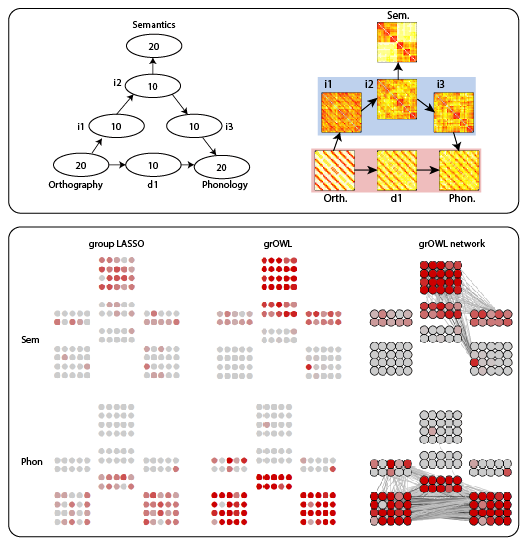
\includegraphics[width=0.75\textwidth]{Network_results.png}
\caption{Top panel: Network architecture (left) and the similarity structure expressed in each layer (right). Red background shows the direct pathway and blue the indrect pathway from orthography to phonology. Layers in the two pathways encode different similarity structures. The target similarity matrices for the analysis express either the semantic structure (top layer) or the phonological structure (bottom right layer). Arrows indicate feed-forward connectivity. Bottom panel: Units selected by group LASSO (right) and GrOWL (middle) when decoding semantic (top) or phonological (bottom) structure. Colors show the proportion of times across subjects and unit concatenations that the unit received a non-zero weight, with red indicating 1 and gray 0. The rightmost plots show the largest weights in the associated matrix W for each GrOWL model, which pick out two subnetworks in the model.}
\label{fig.network}
\end{figure*}  

  
\begin{figure*}[!t]
\centering
\subfloat[]{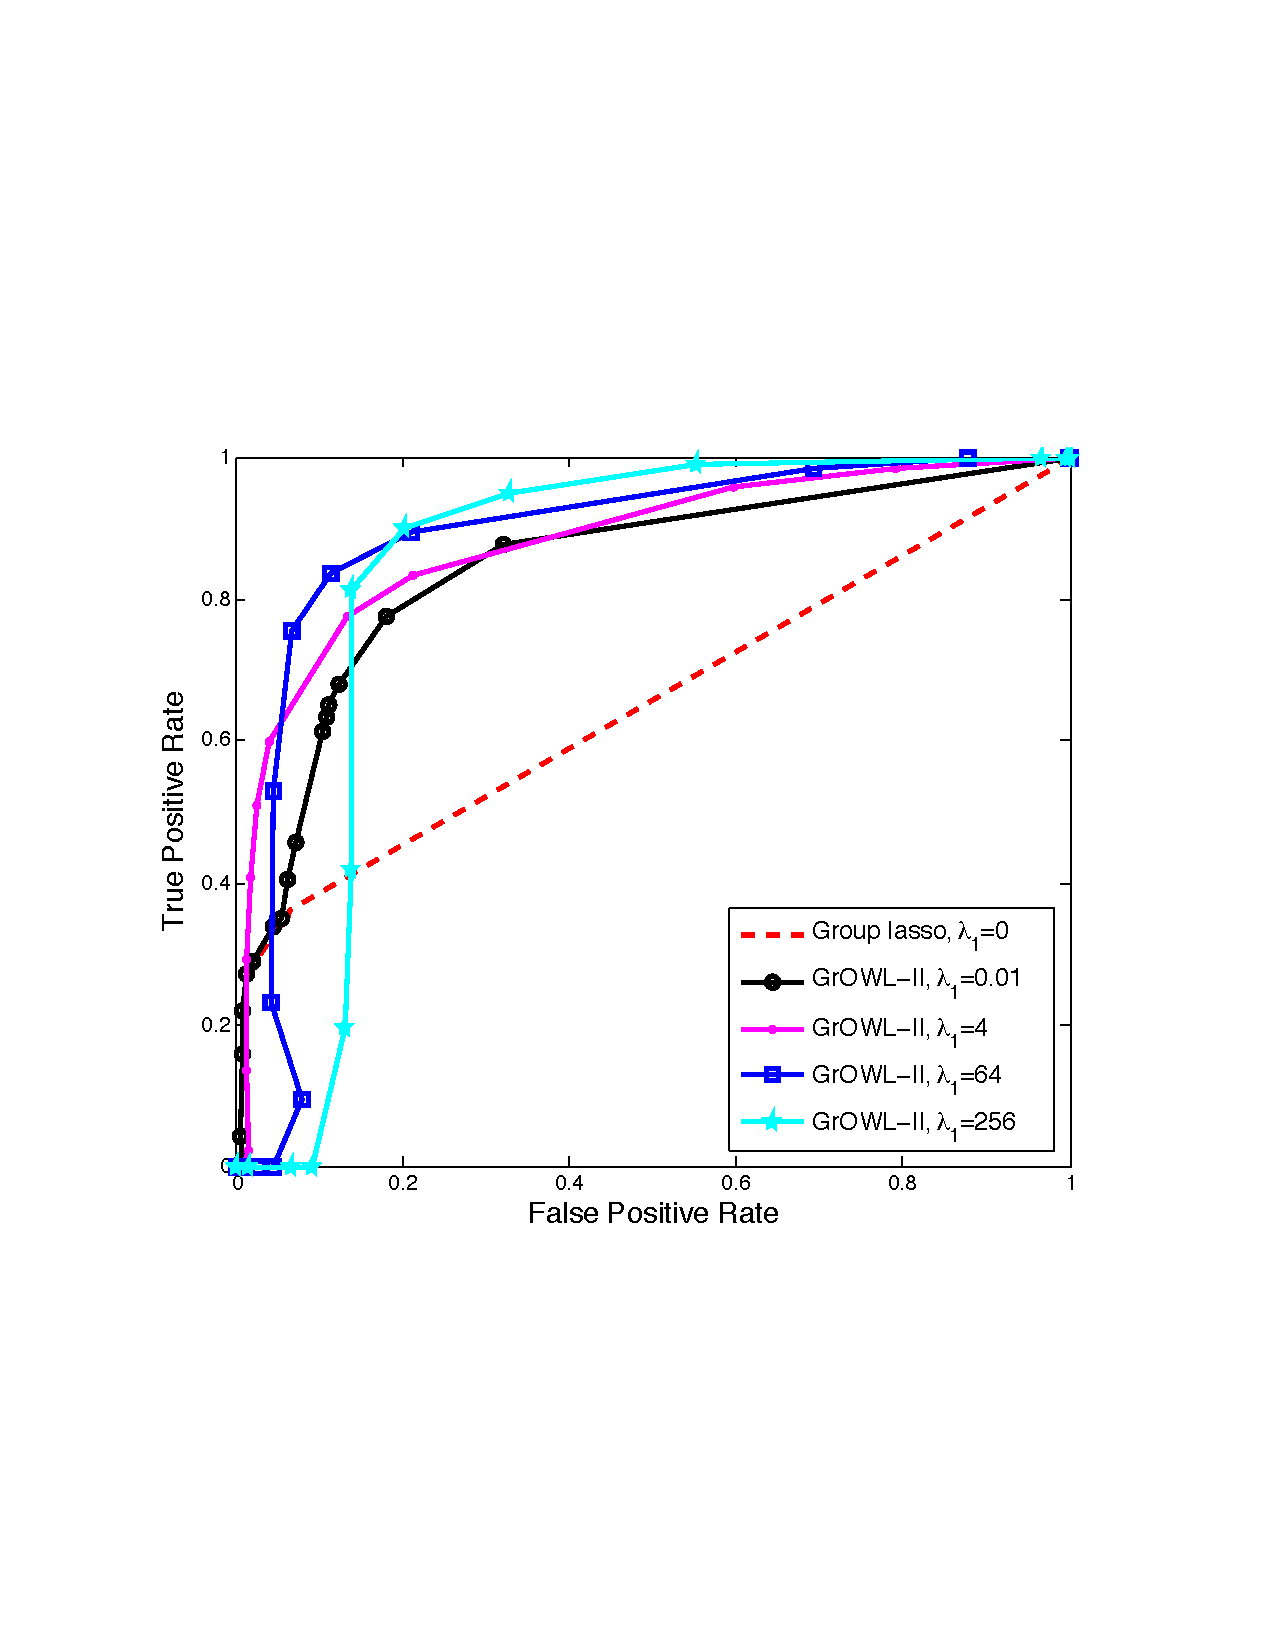
\includegraphics[width=0.45\textwidth]{ROC_sem.pdf}
\label{fig_first_case}}
\hfil
\subfloat[]{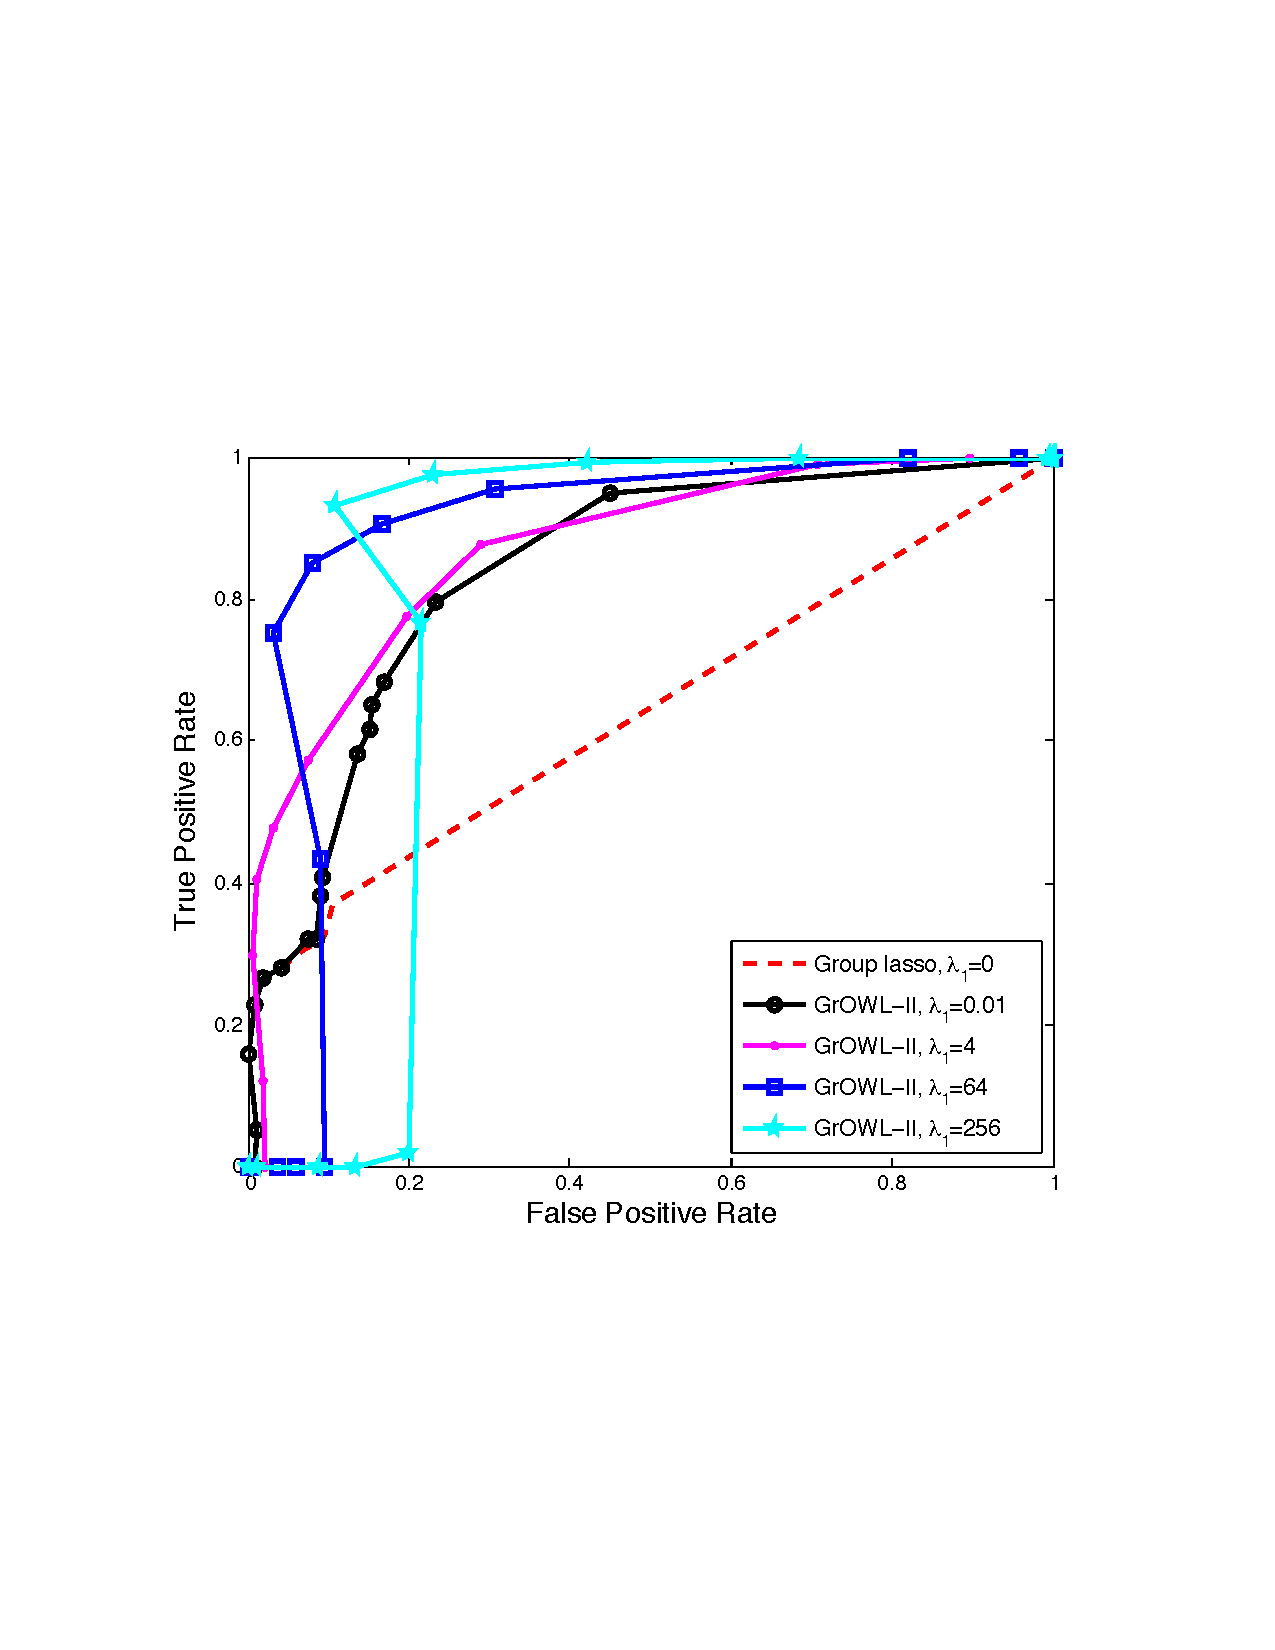
\includegraphics[width=0.45\textwidth]{ROC_phon.pdf}
\label{fig_second_case}}
\caption{ROC curves generated by sweeping through $\lambda$ values (for $\lambda = 0$, all units are selected and as $\lambda$ is increased fewer units are given non-zero weight). Each curve represents a fixed value of $\lambda_1$, where the curve $\lambda_1 = 0$ corresponds to group lasso. ROC curves are averaged across participants for each method, considering both similarity structures, Semantics (left panel) and Phonology (right panel).}
\label{fig.roc}
\end{figure*}



  